\documentclass[12pt,aspectratio=169]{beamer}
\usepackage{talk}

\begin{document}

\title{Using tasks to simplify concurrency in modern C\texttt{++}}  
\author{Christian Blume, Serato}
\date{October 26, 2017 at Pacific\texttt{++}}
% 60 min talk excluding questions

\begin{frame}
\titlepage
\end{frame}

\begin{frame}[fragile]
\frametitle{What is a task?}
A unit of work that \textit{may} be dependent on other tasks.

\bigskip
\bigskip

Examples
\begin{itemize}
\item Adding two numbers
\item Computing a Fourier transformation
\item Making a web request
\item Scheduling a GPU job
\item \ldots
\end{itemize}

\bigskip
\bigskip

In this talk, all tasks are organized in a directed acyclic graph.

\end{frame}

\begin{frame}[fragile]
\frametitle{A simple graph of tasks}
\begin{center}
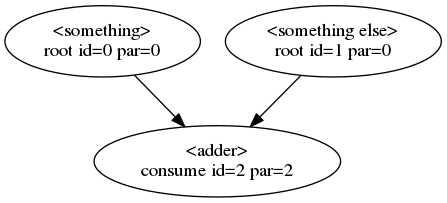
\includegraphics[width=0.7\textwidth]{img/basic_with_three_tasks}
\end{center}
\begin{itemize}
\item parents are at the top ($<$something$>$, $<$something else$>$)
\item parents are consumed or waited for by child ($<$adder$>$)
\item parents are independent with regard to child and can run in parallel
\end{itemize}
\end{frame}

\begin{frame}[fragile]
\frametitle{Task-based concurrency}

\begin{itemize}
\item is concerned with units of work only, not threads
\item is orthogonal to threads, i.e. independent of particular threads
\item allows us to focus on getting stuff done (no thread handling)
\item lets us organize our work into logical, possibly dependent tasks (parallel by design)
\end{itemize}
\bigskip
\bigskip

Disclaimer: Task-based concurrency does NOT help with data races.

\end{frame}

\begin{frame}[fragile]
\frametitle{Two concurrency problems}

\begin{lstlisting}
int x = 0;

void add_one() {
    x += 1;
}

void mult_two() {
    x *= 2;
}
\end{lstlisting}

We want to achieve two goals:
\begin{enumerate}
\item Repeatedly run \lstinline{add_one} on a different thread
\item Repeatedly run \lstinline{add_one} and then \lstinline{mult_two}, both on separate threads
\end{enumerate}
\medskip

Three libraries are compared: standard lib, boost, transwarp
\end{frame}

\begin{frame}[fragile]
\frametitle{Problem 1: Run \lstinline{add_one} only (\textit{classic} approach)}

All code that follows is in a single translation unit. \newline
We're ignoring exception handling.

\bigskip
\bigskip

\begin{lstlisting}
bool quit = false; // do we want to quit processing?
atomic_bool done{false}; // has the result been computed?
bool start = false; // can we start processing?
condition_variable cv; // to notify the worker thread
mutex m; // need this for cv and start
\end{lstlisting}

\bigskip
\bigskip

Please do NOT write code like this!

\end{frame}

\begin{frame}[fragile]
\frametitle{Problem 1: Run \lstinline{add_one} only (\textit{classic} approach)}

\begin{lstlisting}
void worker() { // run on a separate thread
    for (;;) {
        {
            unique_lock<mutex> lock(m);
            cv.wait(lock, [&]{ return start || quit; });
            if (quit) return; // the app wants to terminate
            start = false;
        }
        add_one();
        done = true; // signal that result is available
    }
}
\end{lstlisting}

\end{frame}

\begin{frame}[fragile]
\frametitle{Problem 1: Run \lstinline{add_one} only (\textit{classic} approach)}

\begin{lstlisting}
int main() {
    thread t{worker}; // launch the thread
    int count = 0;
    while (count++ < 3) {
        {
            lock_guard<mutex> lock(m);
            start = true; // we want to start calculating
        }
        cv.notify_one(); // notify to start calculating
        while (!done); // block until result is available (cv?)
        done = false;
        cout << "x = " << x << endl;
    } // end of while
    ...
\end{lstlisting}

\end{frame}

\begin{frame}[fragile]
\frametitle{Problem 1: Run \lstinline{add_one} only (\textit{classic} approach)}

\begin{lstlisting}
    ...
    {
        lock_guard<mutex> lock(m);
        quit = true; // the app is terminated
    }
    cv.notify_one();
    t.join();
}
\end{lstlisting}
\bigskip

Output:
\begin{verbatim}
x = 1
x = 2
x = 3
\end{verbatim}
\end{frame}

\begin{frame}[fragile]
\frametitle{Problem 1: Run \lstinline{add_one} only (\lstinline{std::async} approach)}

\begin{lstlisting}
int main() {
    int count = 0;
    while (count++ < 3) {
        // first param is launch policy
        auto future = async(launch::async, add_one);
        future.wait(); // wait until result becomes available
        cout << "x = " << x << endl;
    }
}
\end{lstlisting}
\bigskip

Problem: No control over the thread that is used to run the operation.

Worst case: Every iteration launches a new thread :(
\end{frame}

\begin{frame}[fragile]
\frametitle{Problem 1: Run \lstinline{add_one} only (\textit{boost} approach)}

\begin{lstlisting}
int main() {
    boost::basic_thread_pool executor{4}; // pool with 4 threads
    int count = 0;
    while (count++ < 3) {
        auto future = boost::async(executor, add_one);
        future.wait();
        cout << "x = " << x << endl;
    }
}
\end{lstlisting}
\bigskip

The custom executor gives us control over where our tasks are executed.

A boost executor can be any class that implements:
\begin{lstlisting}
void submit(boost::function<void()> functor);
\end{lstlisting}
\end{frame}

\begin{frame}[fragile]
\frametitle{Problem 1: Run \lstinline{add_one} only (\textit{transwarp} approach)}

\begin{lstlisting}
int main() {
    tw::parallel executor{4}; // thread pool with 4 threads
    // first param is the task type (root, consume, wait)
    auto task = tw::make_task(tw::root, add_one);
    int count = 0;
    while (count++ < 3) {
        task->schedule(executor);
        task->get_future().wait();
        cout << "x = " << x << endl;
    }
}
\end{lstlisting}

A transwarp executor must implement this interface:
\begin{lstlisting}
string get_name() const;
void execute(const function<void()>& functor, 
             const shared_ptr<tw::node>& node);
\end{lstlisting}
\end{frame}

\begin{frame}[fragile]
\frametitle{Problem 2: Run \lstinline{add_one} and \lstinline{mult_two}}

Given these functions:

\begin{lstlisting}
int x = 0;

void add_one() {
    x += 1;
}

void mult_two() {
    x *= 2;
}
\end{lstlisting}
\medskip

We want to repeatedly run \lstinline{add_one} and then \lstinline{mult_two}, both on separate threads

\end{frame}

\begin{frame}[fragile]
\frametitle{Problem 2: Run \lstinline{add_one} and \lstinline{mult_two} (\textit{classic} approach)}

Not shown to prevent brain injuries.

\bigskip
\bigskip

Essentially:
\begin{itemize}
\item Another set of locks, mutexes, and condition variables
\item Another worker function to wait for \lstinline{add_one} and then run \lstinline{mult_two}
\item Another thread that runs the second worker function
\end{itemize}
\bigskip
\bigskip

Output:
\begin{verbatim}
x = 2
x = 6
x = 14
\end{verbatim}
\end{frame}

\begin{frame}[fragile]
\frametitle{Problem 2: Run \lstinline{add_one} and \lstinline{mult_two} (\textit{boost} approach)}

\begin{lstlisting}
int main() {
    boost::basic_thread_pool executor{4};
    int count = 0;
    while (count++ < 3) {
        auto future1 = boost::async(executor, add_one);
        // make use of a continuation
        auto future2 = future1.then(executor, 
                       [](boost::future<void>) { mult_two(); });
        future2.wait();
        cout << "x = " << x << endl;
    }
}
\end{lstlisting}

This cannot be done with current standard C\texttt{++} but \textit{may} be coming with C\texttt{++}20 (concurrency ts).

\end{frame}

\begin{frame}[fragile]
\frametitle{Problem 2: Run \lstinline{add_one} and \lstinline{mult_two} (\textit{transwarp} approach)}

\begin{lstlisting}
int main() {
    tw::parallel executor{4};
    // build the task graph upfront
    auto task1 = tw::make_task(tw::root, add_one);
    auto task2 = tw::make_task(tw::wait, mult_two, task1);
    int count = 0;
    while (count++ < 3) {
        // schedule all tasks in the right order
        task2->schedule_all(executor); 
        task2->get_future().wait();
        cout << "x = " << x << endl;
    }
}
\end{lstlisting}

\end{frame}

\begin{frame}[fragile]
\frametitle{What we've seen so far}

\begin{itemize}
\item Solved two very simple concurrency problems
\item Four approaches: classic, std::async, boost, transwarp
\end{itemize}

\bigskip

classic approach:
\begin{itemize}
\item Involves locks, mutexes, and condition variables
\item Complicated and error-prone, explicit thread-handling
\item Threads are bound to functions we want to calculate
\item Hard to extend when dependencies change
\end{itemize}
\end{frame}

\begin{frame}[fragile]
\frametitle{Task-based approaches}

std::async approach:
\begin{itemize}
\item Already makes codes much simpler
\item Gives up control of which thread is used to run the operation
\item Cannot be used to model dependencies (Problem 2 cannot be tackled)
\end{itemize}
\medskip

boost approach:
\begin{itemize}
\item Solves the shortcomings of the current C\texttt{++} standard
\item Has support for executors to control where operations are run
\item Allows to model dependencies via future continuations
\end{itemize}
\medskip

transwarp approach:
\begin{itemize}
\item Similar to boost except that tasks can be scheduled multiple times
\item The task graph is built upfront as a model of the operations
\end{itemize}
\end{frame}

\begin{frame}[frame]
\frametitle{Other libraries for task-parallelism}

HPX (High Performance ParalleX)
\begin{itemize}
\item Very similar interface to Boost with regard to futures
\item Neither HPX nor Boost provide task graphs for multiple invocations
\end{itemize}
\bigskip

TBB (Threading Building Blocks)
\begin{itemize}
\item tasks can be chained similar to continuations, also for multiple invocations
\item API seems somewhat harder to use than HPX or Boost
\end{itemize}
\bigskip

Stlab
\begin{itemize}
\item Provides Boost-like future support for one-shot graphs
\item Introduces the concept of \textit{channels} for multiple invocations
\end{itemize}

\end{frame}


\begin{frame}[fragile]
\frametitle{A more evolved problem}

\begin{itemize}
\item Draw random values from a gamma distribution
\item Compute average, standard deviation, mode, and median
\item Goal: Compute stuff in parallel in a task-based fashion
\end{itemize}
\bigskip

The standard deviation:
\begin{equation*}
\sigma = \sqrt{\frac{1}{N} \sum_{i=1}^N (x_i - \overline{x})^2}
\end{equation*}
depends on the average $\overline{x}$ itself!

\end{frame}

\begin{frame}[fragile]
\frametitle{Task graph (courtesy of transwarp)}
\begin{center}
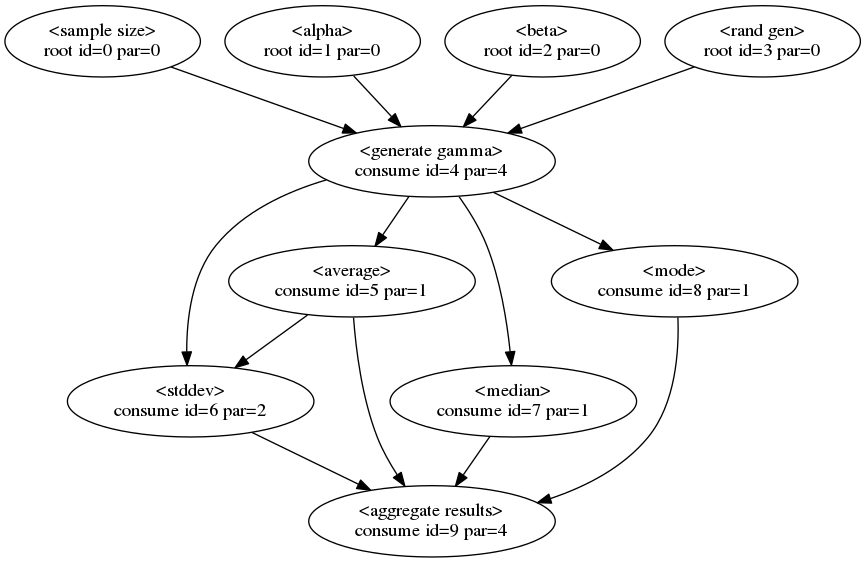
\includegraphics[width=0.85\textwidth]{img/statistical_key_facts}
\end{center}
\end{frame}

\begin{frame}[fragile]
\frametitle{Prerequisites}
\begin{lstlisting}
using data_t = shared_ptr<vector<double>>;

data_t generate_gamma(size_t sample_size, double alpha, 
                      double beta, shared_ptr<mt19937> gen);

double average(data_t data);

double stddev(data_t data, double average);

double median(data_t data);

int mode(data_t data);

// result is a simple struct holding the results
result aggregate(double avg, double std, double med, int mode);
\end{lstlisting}
\end{frame}

\begin{frame}[fragile]
\frametitle{Solving it with Boost}
\begin{lstlisting}
double alpha = 1;
double beta = 1;
boost::basic_thread_pool exec{4};

double count = 1;
while (count < 4) {
    // compute_graph is where the magic happens
    auto future = compute_graph(exec, sample_size, alpha, beta);
    const result res = future.get();
    cout << res << endl;
    // Changing input
    alpha += count;
    beta += count;
    ++count;
}
\end{lstlisting}
\end{frame}

\begin{frame}[fragile]
\frametitle{Solving it with Boost (cont.)}
\begin{lstlisting}
template<typename Executor>
boost::future<result> compute_graph(Executor& exec, 
          size_t sample_size, double alpha, double beta) {
// wrapping parameters into ready futures
auto gen_fut = boost::make_ready_future(make_shared<mt19937>(1));
auto size_fut = boost::make_ready_future(sample_size);
auto alpha_fut = boost::make_ready_future(alpha);
auto beta_fut = boost::make_ready_future(beta);
// creating a future of futures
auto para_fut = boost::when_all(move(gen_fut), move(size_fut), move(alpha_fut), move(beta_fut));
...
\end{lstlisting}
\end{frame}

\begin{frame}[fragile]
\frametitle{Solving it with Boost (cont.)}
\begin{lstlisting}
// Generate the data from a gamma distribution
auto data_fut = para_fut.then(exec, [](decltype(para_fut) f) {
    auto p = f.get(); // p is a tuple of futures
    shared_ptr<mt19937> gen = get<0>(p).get();
    size_t sample_size = get<1>(p).get();
    double alpha = get<2>(p).get();
    double beta = get<3>(p).get();
    return generate_gamma(sample_size, alpha, beta, gen);
}).share();
// Compute the average
auto avg_fut = data_fut.then(exec, [](boost::shared_future<data_t> f) {
    return average(f.get());
}).share();
...
\end{lstlisting}
\end{frame}

\begin{frame}[fragile]
\frametitle{Solving it with Boost (cont.)}
\begin{lstlisting}
// future of futures that waits for completion of parents
auto d_a_fut = boost::when_all(data_fut, avg_fut);
// Compute the stddev using data and average
auto stddev_fut = d_a_fut.then(exec, [](decltype(d_a_fut) f) {
    auto data_avg = f.get(); // data_avg is a tuple of futures
    data_t data = get<0>(data_avg).get();
    double avg = get<1>(data_avg).get();
    return stddev(data, avg);
});
// Compute the median
auto median_fut = data_fut.then(exec, [](boost::shared_future<data_t> f) {
    return median(f.get());
});
...
\end{lstlisting}
\end{frame}

\begin{frame}[fragile]
\frametitle{Solving it with Boost (cont.)}
\begin{lstlisting}
// Compute the mode
auto mode_fut = data_fut.then(exec, [](boost::shared_future<data_t> f) {
    return mode(f.get());
});
// Wait for all to finish
auto agg_wait_fut = boost::when_all(avg_fut, move(stddev_fut), move(median_fut), move(mode_fut));
// Create aggregated result
return agg_wait_fut.then(exec, [](decltype(agg_wait_fut) f){
    auto r = f.get(); // r is a tuple of futures
    return aggregate(get<0>(r).get(), get<1>(r).get(), 
                     get<2>(r).get(), get<3>(r).get());
});
} // compute_graph
\end{lstlisting}
\end{frame}

\begin{frame}[fragile]
\frametitle{Solving it with transwarp}
\begin{lstlisting}
double alpha = 1;
double beta = 1;
// Creating the task graph upfront
auto task = build_graph(sample_size, alpha, beta);
tw::parallel exec{4};
double count = 1;
while (count < 4) {
    task->schedule_all(exec); // schedule all in the right order
    const result res = task->get_future().get();
    cout << res << endl;
    // Changing input
    alpha += count;
    beta += count;
    ++count;
}
\end{lstlisting}
\end{frame}

\begin{frame}[fragile]
\frametitle{Solving it with transwarp (cont.)}
\begin{lstlisting}
shared_ptr<tw::task<result>> build_graph(size_t sample_size, 
                               double& alpha, double& beta) {
auto gen = make_shared<mt19937>(1);
// Creating parameter tasks at the top of the graph
auto gen_task = tw::make_task(tw::root, [gen] { return gen; });
auto size_task = tw::make_task(tw::root, 
                        [sample_size] { return sample_size; });
auto alpha_task = tw::make_task(tw::root, 
                               [&alpha] { return alpha; });
auto beta_task = tw::make_task(tw::root, 
                               [&beta] { return beta; });
// The data task consumes the parameter tasks
auto data_task = tw::make_task(tw::consume, generate_gamma, 
                 size_task, alpha_task, beta_task, gen_task);
...
\end{lstlisting}
\end{frame}

\begin{frame}[fragile]
\frametitle{Solving it with transwarp (cont.)}
\begin{lstlisting}
// Create tasks for the different measures
auto avg_task = tw::make_task(tw::consume, average, data_task);
auto stddev_task = tw::make_task(tw::consume, stddev, 
                                 data_task, avg_task);
auto median_task = tw::make_task(tw::consume, median, 
                                 data_task);
auto mode_task = tw::make_task(tw::consume, mode, data_task);
// Create the final aggregate task
shared_ptr<tw::task<result>> t = tw::make_task(tw::consume, aggregate, avg_task, stddev_task, median_task, mode_task);
return t;
} // build_graph
\end{lstlisting}
\end{frame}

\begin{frame}[fragile]
\frametitle{Conclusions}
We've seen
\begin{itemize}
\item two very simple concurrency problems
\item a real-world case study from statistics
\end{itemize}
\bigskip

Take away
\begin{itemize}
\item task-based approaches greatly simplify concurrent code
\item task-based concurrency is orthogonal to threads
\item futures in current standard are pretty weak (hopefully better in C\texttt{++}20)
\item Boost futures allow for continuations with custom executors
\item transwarp further simplifies task-based concurrency 
\item transwarp provides a task-graph for multiple invocations
\item other great libraries: HPX, TBB, Stlab, etc.
\end{itemize}
\end{frame}

\begin{frame}[fragile]
\huge
\begin{center}
Thank You
\end{center}
\end{frame}

\begin{frame}[fragile]
\frametitle{transwarp - future work}
\begin{itemize}
\item Add new methods to \lstinline{task}: \lstinline{wait()}, \lstinline{get()}
\item Create function to create a \textit{ready} task with given value
\item Create custom \lstinline{packaged_task} for better scheduling performance
\item Improve error messages, in particular when parent tasks don't match the child task
\item \ldots
\end{itemize}
\bigskip
\bigskip
I am accepting pull requests!
\bigskip

\url{https://github.com/bloomen/transwarp}
\bigskip

\end{frame}

\begin{frame}[fragile]
\frametitle{\lstinline{schedule_impl(tw::executor* executor)}}
\begin{lstlisting}
weak_ptr<task_impl> self = this->shared_from_this();
auto futures = tw::detail::get_futures(parents_);
auto pack_task = make_shared<packaged_task<result_type()>>(bind( &task_impl::evaluate, node_->get_id(), move(self), move(futures)));
future_ = pack_task->get_future();
if (executor_) {
    executor_->execute([pack_task] { (*pack_task)(); }, node_);
} else if (executor) {
    executor->execute([pack_task] { (*pack_task)(); }, node_);
} else {
    (*pack_task)();
}
\end{lstlisting}
\end{frame}

\begin{frame}[fragile]
\frametitle{transwarp}
\begin{center}

\includegraphics[width=0.8\textwidth]{img/transwarp_conduit}
\end{center}
\end{frame}

\end{document}
